%!TEX root = *.tex
%%%%%%%%%%%%%%%%%%
% カウンタのリセット
% 問題文
{\begin{wrapfigure}{r}{12zw}
  \vspace*{-\intextsep}
  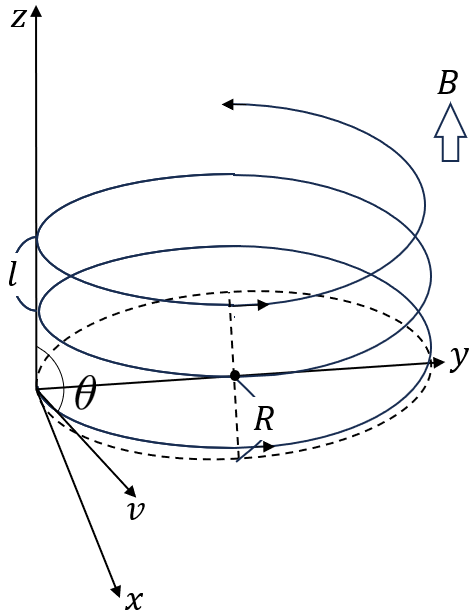
\includegraphics[width=12zw]{../graphs/jumon_123.png}
\end{wrapfigure}
真空中に一様な磁束密度$B\unit{T}$の磁場がある.
図に示すように,\xyz 軸をとる.
磁場の方向は\z 軸とする.
その磁場の中に速さ\mbox{$v\unit{m/s}$}の電子(質量$m\unit{kg}$,電荷$-e\unit{C}$)を\zx 平面上で,\z 軸の正の向きに対して$\theta\,(<90^\circ)$の角度で入射させる.
この点を原点Oとする.
ただし,電子は原点Oを通過後から磁場の影響を受けた運動をするものとする.

\begin{enumerate}[(1)]
  \setlength{\leftskip}{-1.5zw}
  \setlength{\itemindent}{1zw}\setlength{\labelsep}{0.5zw}
  \setlength{\labelwidth}{1zw}\setlength{\leftmargin}{1zw}
  \setlength{\itemsep}{0.5\baselineskip}
  \item 電子が原点Oに入射したとき,電子の速さの\y 成分は0である.\x 成分と\z 成分を求めよ.
  \item 電子が磁場から受ける力の大きさ$F\unit{N}$を求めよ.
\end{enumerate}

\par}
\begin{enumerate}[(1)]
  \setlength{\leftskip}{-1.5zw}
  \setlength{\itemindent}{1zw}\setlength{\labelsep}{0.5zw}
  \setlength{\labelwidth}{1zw}\setlength{\leftmargin}{1zw}
  \setlength{\itemsep}{0.5\baselineskip}
  \setcounter{enumi}{2}
  \item 電子が磁場から受ける力は,大きさが一定で電子の運動方向と常に垂直にはたらく.電子は磁場に垂直な平面内で等速円運動を行うので,\z 軸方向から見たとき図の破線のような半径$R\unit{m}$の等速円運動を行う.円運動の半径$R$を求めよ.
  \item $R$を用いずに円運動の周期$T\unit{s}$を表せ.
  \item \z 軸方向の運動は(1)で答えた入射の速さを変えずに運動する.(3)と合わせて,電子の運動は磁場の向きを軸としたらせん運動となる.図に示すらせん運動のピッチ$l\unit{m}$を求めよ.
  \item 原点Oに入射する電子を初速0から電位差$E\unit{V}$で加速した.このときの電子の速さ$v$を$m,\,e,\,E$で表せ.
  \item 比電荷$\dfrac{e}{m}\unit{C/kg}$を$R,\,E,\,B,\,\theta$で表せ.
\end{enumerate}


% メモ
\begin{comment}

\end{comment}


%%%%%%%%%%%%%%%%%%
